\documentclass{standalone}
\usepackage{tikz}
\usepackage{ctex,siunitx}
\usepackage{tkz-euclide}
\usepackage{amsmath}
\usetikzlibrary{patterns, calc}
\usetikzlibrary {decorations.pathmorphing, decorations.pathreplacing, decorations.shapes,}
\begin{document}
\small
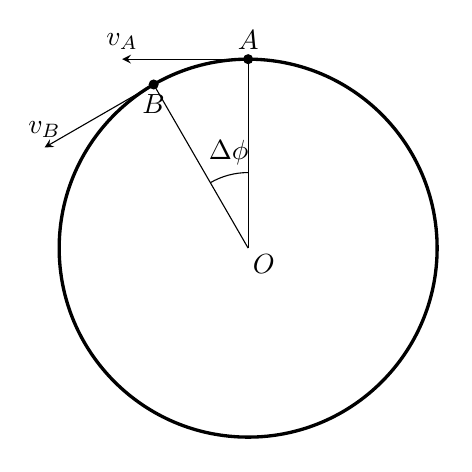
\begin{tikzpicture}[>=stealth,scale=0.8]
  \useasboundingbox(-3.5,-3.1)rectangle(3.1,3.5);
  \draw [very thick](0,0)  circle [radius=3];
  \node at (.25,-.25){$O$};
  \draw (0,0)--(90:3) node [above]{$A$};
  \draw (0,0)--(120:3) node [below]{$B$};
  \draw [fill=black] (90:3) circle (2pt) ;
  \draw [fill=black] (120:3) circle (2pt) ;
  \draw (0,0+1.2) arc (90:120:1.2) node [midway,above]{$\Delta \phi$};
  \draw [<-](-2,3)node [above]{$v_A$}--(0,3);
  \draw [->](120:3)--+(120+90:2)node [above]{$v_B$};
\end{tikzpicture}
\end{document}